\documentclass[12pt, letterpaper]{article}
\usepackage{amsmath,amssymb,amsthm,amsopn,amscd}
\usepackage{mathtools}
\usepackage{latexsym}
\usepackage{graphicx,caption,subcaption}
\usepackage{multirow}
\usepackage[reftex]{theoremref}
\usepackage{hyperref}
\usepackage{verbatim}
\usepackage{color}
\usepackage{algorithm}      % pseudo-code
\usepackage{algpseudocode}  %
\usepackage{stmaryrd}       % double brackets
\usepackage{amstext}    % \text macro
\usepackage{array}      % \newcolumntype macro
\usepackage{tikz}       % for flow chart
\usetikzlibrary{cd}     % commutative diagram
\usetikzlibrary{shapes.geometric} % pentagon
\usetikzlibrary{calc}
\usetikzlibrary{patterns}
\usepackage{graphics, tkz-berge} % icosahedron
\usepackage{afterpage}
\usepackage[export]{adjustbox}
\usepackage{tensor}
\usepackage{braket}
\usepackage{etoolbox}
\usepackage{xparse}
\usepackage{titlesec}	% lv4 title
%\usepackage{subfigure}
\usepackage{mathrsfs}
\usepackage{pgfplots}
%   \usepackage{commath}    % for abs and norm

\usepackage{ytableau}
%\usepackage{geometry}		% change margin
\usepackage[margin=1.5in]{geometry} 		% change margin

%\setcounter{secnumdepth}{-2} % remove section numbering
\setcounter{section}{-1}

%\newcommand{\executeiffilenewer}[3]{%
%	\ifnum\pdfstrcmp{\pdffilemoddate{#1}}%
%	{\pdffilemoddate{#2}}>0%
%	{\immediate\write18{#3}}\fi%
%}
%\newcommand{\includesvg}[1]{%
%	\executeiffilenewer{#1.svg}{#1.pdf}%
%	{inkscape -z -D --file=#1.svg %
%		--export-pdf=#1.pdf --export-latex}%
%	\input{#1.pdf_tex}%
%}



\graphicspath{ {./} }

\makeatletter
\renewcommand\subparagraph{\@startsection{subparagraph}{5}{\parindent}%
	{3.25ex \@plus1ex \@minus .2ex}%
	{0.75ex plus 0.1ex}% space after heading
	{\normalfont\normalsize\bfseries}}
\makeatother

\newcommand\independent{\protect\mathpalette{\protect\independenT}{\perp}}
\def\independenT#1#2{\mathrel{\rlap{$#1#2$}\mkern2mu{#1#2}}}
\newcommand{\rp}{\mathbb{RP}}

\newcommand{\transpose}[1]{{{#1}^{\intercal}}}

%   Sets

\newcommand{\calS}{\mathcal{S}}
\newcommand{\calT}{\mathcal{T}}

\newcommand{\nat}{\mathbb{N}}
\newcommand{\inte}{\mathbb{Z}}
\newcommand{\rat}{\mathbb{Q}}
\newcommand{\re}{\mathbb{R}}
\newcommand{\renn}{\mathbb{R}_0^+}
\newcommand{\co}{\mathbb{C}}
\newcommand{\hil}{\mathbb{H}}
\newcommand{\field}{\mathbb{F}}
\newcommand{\ee}{\mathrm{e}}
\newcommand{\dd}{\mathrm{d}}
\newcommand{\GL}{\operatorname{GL}}
\newcommand{\SL}{\operatorname{SL}}
\newcommand{\PGL}{\operatorname{PGL}}
\newcommand{\PSL}{\operatorname{PSL}}
\newcommand{\MM}{\operatorname{M}}
\newcommand{\ZZ}{\operatorname{Z}}
\newcommand{\SZ}{\operatorname{SZ}}
\newcommand{\ob}{\operatorname{ob}}
\newcommand{\dom}{\operatorname{dom}}
\newcommand{\cod}{\operatorname{cod}}
\newcommand{\Hom}{\operatorname{Hom}}
\newcommand{\End}{\operatorname{End}}
\newcommand{\class}{\operatorname{class}}
\newcommand{\supp}{\operatorname{supp}}
\newcommand{\idt}{\operatorname{id}}
\newcommand{\sgn}{\operatorname{sgn}}
\newcommand{\Sym}{\operatorname{Sym}}
\newcommand{\Tr}{\operatorname{Tr}}
\newcommand{\Cl}{\operatorname{Cl}}
\newcommand{\Res}{\operatorname{Res}}
\newcommand{\Ind}{\operatorname{Ind}}

\newcommand{\ext}[1]{\bigwedge\!^{#1}}


\DeclarePairedDelimiter\ceil{\lceil}{\rceil}
\DeclarePairedDelimiter\floor{\lfloor}{\rfloor}


\newcommand{\id}{\indices}
%   \newcommand{\cp}{\mathbb{CP}}
%   \newcommand{\dS}{\mathbb{S}}
%   \newcommand{\dP}{\mathbb{P}}
%   \newcommand{\dE}{\mathbb{E}}
%   \newcommand{\dZ}{\mathbb{Z}}
\newcommand{\rmT}{\mathrm{T}}
\newcommand{\rmR}{\mathrm{R}}
\newcommand{\bfP}{\mathbf{P}}
\newcommand{\bfJ}{\mathbf{J}}
\newcommand{\bfK}{\mathbf{K}}
\newcommand{\bfR}{\mathbf{R}}
\newcommand{\idm}{\mathbf{I}}
\newcommand{\bfA}{\mathbf{A}}
\newcommand{\bfB}{\mathbf{B}}
\newcommand{\bfC}{\mathbf{C}}
\newcommand{\bfD}{\mathbf{D}}
\newcommand{\bfG}{\mathbf{G}}
\newcommand{\bfL}{\mathbf{L}}
\newcommand{\bfT}{\mathbf{T}}
\newcommand{\bfS}{\mathbf{S}}
\newcommand{\bfe}{\mathbf{e}}
%   \newcommand{\bm}{\boldsymbol{m}}
%   \newcommand{\bmu}{\boldsymbol{\mu}}
%   \newcommand{\bS}{\boldsymbol{\Sigma}}
%   \newcommand{\uvec}[1]{\mathrm{\mathbf{\hat{e}}}_#1}
%   \newcommand{\rmbf}[1]{\mathrm{\mathbf{#1}}}
%   \newcommand{\javg}{J_{\mathrm{avg^2}}}
%   \newcommand{\pgl}[1]{\mathbf{PGL}(#1,\mathbb{R})}
%   \newcommand{\Sl}[1]{\mathbf{SL}(#1,\mathbb{R})}
%   \newcommand{\gl}[1]{\mathbf{GL}(#1,\mathbb{R})}

\makeatletter
\newcommand\etc{etc\@ifnextchar.{}{.\@}}
\newcommand\ie{i.e\@ifnextchar.{}{.\@}}
\newcommand\eg{e.g\@ifnextchar.{}{.\@}}
\newcommand\Eq{Eq.\ }
\makeatother


\NewDocumentCommand\closure{sm}
{\IfBooleanTF{#1}{\overline{#2}}{\overline{#2}}}
\NewDocumentCommand\interior{sm}
{\IfBooleanTF{#1}{?}{\mathring{#2}}{}}

\newcommand{\red}[1]{{\color{red} #1}}
\newcommand{\blue}[1]{{\color{blue} #1}}		

\newcommand{\power}{\mathcal{P}}
\newcommand{\domain}{\mathcal{D}}

\newcommand{\opp}[1]{{#1}^{\mathrm{op}}}

\newcommand{\na}{\nabla}
\newcommand{\abs}[1]{\left\lvert #1 \right\rvert}
\newcommand{\card}[1]{\left\lvert #1 \right\rvert}
\newcommand{\norm}[1]{\left\lVert #1 \right\rVert}
\newcommand{\gaussian}{\mathcal{N}}
\newcommand{\define}{\coloneqq}
\newcommand{\tp}[1]{{#1}^T}
\newcommand{\hadj}[1]{{#1}^{\dagger}}
\newcommand{\conj}{\overline}
\renewcommand{\emptyset}{\varnothing}
\newcommand{\symdif}{\triangle}
%
%   \newcommand{\lst}[2]{\{#1_{1}, #1_{2}, \dots, #1_{#2}\}}
%   \newcommand{\lstf}[2]{\{#1{1}, #1{2}, \dots, #1{#2}\}}
%   % prt stands for parenthesis
%   \newcommand{\prt}[2]{(#1_{1}, #1_{2}, \dots, #1_{#2})}
%   \newcommand{\prtf}[2]{(#1{1}, #1{2}, \dots, #1{#2})}
%   % general list formatted, #1: fxn, #2: first one, #3: last one, #4: delimiter, #5: left, #6: right
%   \newcommand{\glstf}[6]{#5 #1{#2} #4 #1{\number\numexpr#2+1\relax} #4 \dots #4 #1{#3} #6}
%
% wc = wild card
\newcommand*{\wcthin}{{\mkern 2mu\cdot\mkern 2mu}}
\newcommand*{\wc}{{}\cdot{}}    %   This one is wider
%
% Operators
% ec = equivalence class
\newcommand{\ec}[1]{\left[{#1}\right]}
% generating subgroup
\newcommand{\gensub}[1]{\left\langle{#1}\right\rangle}
%
%   automatic math mode in tabular
\newcolumntype{L}{>{$}l<{$}}
\newcolumntype{C}{>{$}c<{$}}
\newcolumntype{R}{>{$}r<{$}}

\newenvironment{centabular}{\center\tabular}{\endtabular\endcenter}
\newenvironment{centikzpic}{\center\tikzpicture}{\endtikzpicture\endcenter}
\newenvironment{centikzcd}{\center\tikzcd}{\endtikzcd\endcenter}
\newenvironment{eqlong}{\equation\aligned}{\endaligned\endequation}


\DeclareMathOperator*{\argmin}{arg\,min}
\DeclareMathOperator*{\argmax}{arg\,max}
\DeclareMathOperator{\Var}{Var}
\DeclareMathOperator{\Cov}{Cov}
\DeclareMathOperator{\rank}{rank}
\DeclareMathOperator{\spn}{span}
\DeclareMathOperator{\diag}{diag}
\DeclareMathOperator{\tr}{tr}

\newtheorem*{prop*}{Proposition}
\newtheorem{prop}{Proposition}[section]
\newtheorem*{lem*}{Lemma}
\newtheorem{lem}[prop]{Lemma}
\newtheorem{cor}[prop]{Corollary}
\newtheorem{thm}[prop]{Theorem}
\newtheorem*{thm*}{Theorem}
\newtheorem{conjec}[prop]{Conjecture}


%\titleformat{\paragraph}
%{\normalfont\normalsize\bfseries}{\theparagraph}{1em}{}
%\titlespacing*{\paragraph}
%{0pt}{3.25ex plus 1ex minus .2ex}{1.5ex plus .2ex}

%\makeatletter
%\renewcommand\paragraph{\@startsection{paragraph}{4}{\z@}%
%	{3.25ex \@plus1ex \@minus.2ex}%
%	{-1em}%
%	{\normalfont\normalsize\bfseries}}
%\renewcommand\subparagraph{\@startsection{subparagraph}{5}{\parindent}%
%	{3.25ex \@plus1ex \@minus .2ex}%
%	{-1em}%
%	{\normalfont\normalsize\bfseries}}
%%\def\toclevel@subsubsubsection{4}
%\def\toclevel@paragraph{4}
%\def\toclevel@paragraph{5}
%\def\toclevel@definition{6}
%%\def\l@subsubsubsection{\@dottedtocline{4}{7em}{4em}}
%%\def\l@paragraph{\@dottedtocline{4}{10em}{5em}}
%%\def\l@subparagraph{\@dottedtocline{5}{14em}{6em}}
%%\def\l@definition{\@dottedtocline{6}{15em}{7em}}
%\def\l@paragraph{\@dottedtocline{4}{6em}{4em}}
%\def\l@subparagraph{\@dottedtocline{5}{8em}{5em}}
%\def\l@definition{\@dottedtocline{6}{8.5em}{0em}}
%\makeatother
%
%\setcounter{secnumdepth}{6}
%\setcounter{tocdepth}{6}

%https://tex.stackexchange.com/questions/280313/how-to-put-the-list-of-definitions-at-contents-page
%https://tex.stackexchange.com/questions/51691/creating-list-of-for-newtheoremstyle
%\usepackage{amsthm}
%\newtheoremstyle{mystyle}
%{\topsep}{\topsep}{}{}{\bfseries}{:}{\newline}
%{\thmname{#1}\thmnumber{ #2}\thmnote{ (#3)}%
%	\ifstrempty{#3}%
%	{\addcontentsline{def}{subsection}{#1~\thedef}}%
%	{\addcontentsline{def}{subsection}{#1~\thedef~(#3)}}}
%
%\theoremstyle{mystyle}
%\newtheorem*{def*}{Definition}
\theoremstyle{definition}
\newtheorem*{defaux}{Definition}

%https://tex.stackexchange.com/questions/60872/ams-theorems-in-table-of-contents
\NewDocumentEnvironment{def*}{o}
{\IfNoValueTF{#1}
	{\defaux\addcontentsline{toc}{definition}{\protect\numberline{}Definition}}
	{\defaux[#1]\addcontentsline{toc}{definition}{\protect\numberline{}Definition (#1)}}%
	\ignorespaces}
{\label{#1}}
{\enddefaux}

%\makeatletter
%\newcommand\definitionname{Definition}
%\newcommand\listdefinitionname{List of Definitions}
%\newcommand\listofdefinitions{%
%	\section*{\listdefinitionname}\@starttoc{def}}
%\makeatother

\theoremstyle{remark}
\newtheorem*{rem*}{Remark}
\newtheorem*{ack*}{Acknowledgements}

\theoremstyle{definition}
\newtheorem{exe}{Exercise}[section]
\newtheorem{exe*}[exe]{Exercise*}
\newtheorem{exam}[exe]{Example in Book}
\newtheorem{eq}[exe]{Equation in Book}
\newtheorem{ddef}[exe]{Definition in Book}
\theoremstyle{plain}
\newtheorem{pprop}[exe]{Proposition in Book}
\newtheorem{ccor}[exe]{Corollary in Book}
\newtheorem{llem}[exe]{Lemma in Book}
\newtheorem{tthm}[exe]{Theorem in Book}
\captionsetup{width=0.9\textwidth}


%%  \usetikzlibrary{shadows}% for shadow
%%  \tikzstyle{event} = [color=black!40,text=white,text centered,circular drop shadow,font=\large\bfseries,text height=4em,text width=4em]
%   \tikzstyle{event} = [draw, circle]
%   \tikzstyle{arrow} = [thick,->,>=stealth]
%%  \usetikzlibrary{arrows}
%%  \tikzstyle{arrow} = [draw, -latex', thick]
%
%   %only for this doc
%   \newcommand{\llb}{\llbracket}
%   \newcommand{\rrb}{\rrbracket}

%opening
\title{Reading Notes for \\ \large \textit{Category Theory} \\ by Steve Awodey}
\author{Zhi Wang}

\numberwithin{equation}{section}


\begin{document}
	
	\cleardoublepage
	\ytableausetup{centertableaux}
	
	\maketitle
	
	
	% https://tex.stackexchange.com/questions/154464/page-numbering-in-table-of-contents
	
	% Let's change \thepage so it prints one less than
	% the real page number; \pagenumbering{arabic}
	% will redefine it to the right meaning afterwards.
	\renewcommand\thepage{\romannumeral\numexpr\value{page}\relax}
	
	\tableofcontents
	
	%	\listofdefinitions
	
	\cleardoublepage
	\pagenumbering{arabic}
	
	
	\section{Notes and Definitions}
	\subsection{Notes}
	
	\section{Categories}
	\subsection{Introduction}
	\subsection{Functions of sets}
	\subsection{Definition of a category}
	\subsection{Examples of categories}
	\paragraph{1}
	\subparagraph{Functions with fibers of at most 2 elements}
	Assume
	\[\forall A,B\in \bfC\, \forall (f\colon A\to B )\,\Big[
	 \forall b\in B\big(\card{f^{-1}(b)}\le 2\big) \iff f\in \Hom_\bfC(A,B)  \Big].  \]
	
	Given that
	\[ \forall B\in\bfC\forall b\in B \Big[\card{1_B^{-1}(b)}=1\le 2\Big] , \]
	we know 
	\[ \forall B\in\bfC \Big[ 1_B\in\Hom_\bfC(B,B)\Big ]. \]
	
	Given $\forall A,B,C\in \bfC,\forall (f\colon A\to B) \,\forall (g\colon B\to C)$
	\[  \forall b\in B\Big(\card{f^{-1}(b)}\le 2\Big) \land  \forall c\in C\Big(\card{g^{-1}(b)}\le 2\Big) 
	\implies \forall c\in C \Big(\card{(g\circ f)^{-1}(c)}\le 4\Big)
	 \]
	which means that the composite $g\circ f$ does not necessarily exist in $\Hom_\bfC(A,B)$.
	
	Therefore, this is \textbf{not} a category.
	
	%https://tex.stackexchange.com/questions/402265/draw-concentric-boxes-around-elements-of-matrix-tikz
	%https://tex.stackexchange.com/questions/377608/animated-tikz-matrix-inside-a-flowchart-node
	%https://tex.stackexchange.com/questions/408497/box-around-tikz-cd-diagram-without-ampersand-replacement
	%https://tex.stackexchange.com/questions/409076/tikz-matrix-with-dotted-node-borders-but-not-on-the-first-row
	%https://dudebout.com/files/pdfs/matrix.skeleton-manual.pdf
	
	\begin{centikzcd}[remember picture,
		%row 1/.style={
		%	nodes={draw=gray, solid, fill=gray!50!white,font=\bfseries, text centered}}
		%%%%
		%boxedcd={inner sep=1pt}
		%%%%
		every matrix/.append style={column sep=tiny, name=fibertwo
			%, rows={draw=red}
		}]
		a_1\ar[rd,"f"]&&a_2\ar[ld,"f"']&&a_3\ar[rd,"f"]&&a_4\ar[ld,"f"']\\
		&b_1\ar[rrd,"g"]&&&&b_2\ar[lld,"g"']&\\
		&&&c&&&
	\end{centikzcd}
	\begin{tikzpicture}[remember picture, overlay]
		\def\mid{40}
		\draw[blue,rounded corners] ([xshift=0pt]fibertwo.south west) rectangle ([xshift=15pt, yshift=15pt]fibertwo.south east)
		node [black, below left] {$C$};
		\draw[blue,rounded corners] ([xshift=0pt,yshift=37.5 pt]fibertwo.south west) rectangle
		([xshift=15pt, yshift=52.5 pt]fibertwo.south east)
		node [black, below left] {$B$};
		\draw[blue,rounded corners] ([xshift=0pt]fibertwo.north west) rectangle ([xshift=15pt, yshift=-15pt]fibertwo.north east)
		node [black, above left] {$A$};
		% -- ([yshift=0pt]fibertwo.north east) -- ([yshift=0pt]fibertwo.north west) -- cycle; 
	\end{tikzpicture}

	\subparagraph{Functions with finite fiber}
	Assume
	\[\forall A,B\in \bfC\, \forall (f\colon A\to B )\,\Big[
	\forall b\in B\big(\card{f^{-1}(b)} \in\nat \big) \iff f\in \Hom_\bfC(A,B)  \Big].  \]
	
	Given that
	\[ \forall B\in\bfC\forall b\in B \Big[\card{1_B^{-1}(b)}=1\in \nat\Big] , \]
	we know 
	\[ \forall B\in\bfC \Big[ 1_B\in\Hom_\bfC(B,B)\Big ]. \]
	
	Given $\forall A,B,C\in \bfC,\forall (f\colon A\to B) \,\forall (g\colon B\to C)$
	\[  \forall b\in B\Big(\card{f^{-1}(b)}\in\nat\Big) \land  \forall c\in C\Big(\card{g^{-1}(b)}\in\nat\Big) 
	\iff \forall c\in C \Big(\card{(g\circ f)^{-1}(c)}\in\nat\Big)
	\]
	since the multiplication of finite numbers are finite, and converse is true.
	This means that the composite $g\circ f$ must exist in $\Hom_\bfC(A,B)$.
	
	Therefore, this \textbf{is} a category.
	
	\subparagraph{Functions with infinite fiber}
	Since identity map has finite fiber, this is \textbf{not} a category.
	
	\paragraph{2}
	\begin{itemize}
		\red{
		\item graphs and graph homomorphisms
		\item the real numbers $R$ and continuous functions $R \to R$,
		\item the natural numbers $N$ and all recursive functions $N \to N$, or as in
		the example of continuous functions, one can take partial recursive
		functions defined on subsets $U \subseteq N$}
	\end{itemize}
	%\setcounter{section}{10}
	\paragraph{11}
	
	\red{Category of data types and programs}
	
	Let's define a procedure as
	\texttt{
		Int f(Int a, Int b) {
			return a * b;
		}
	}

	We have built a morphism/arrow
	
	\[\texttt{f}\colon \texttt{Int}\times \texttt{Int}\to \texttt{Int}.\]
	
	\begin{figure}[H]
		\centering
		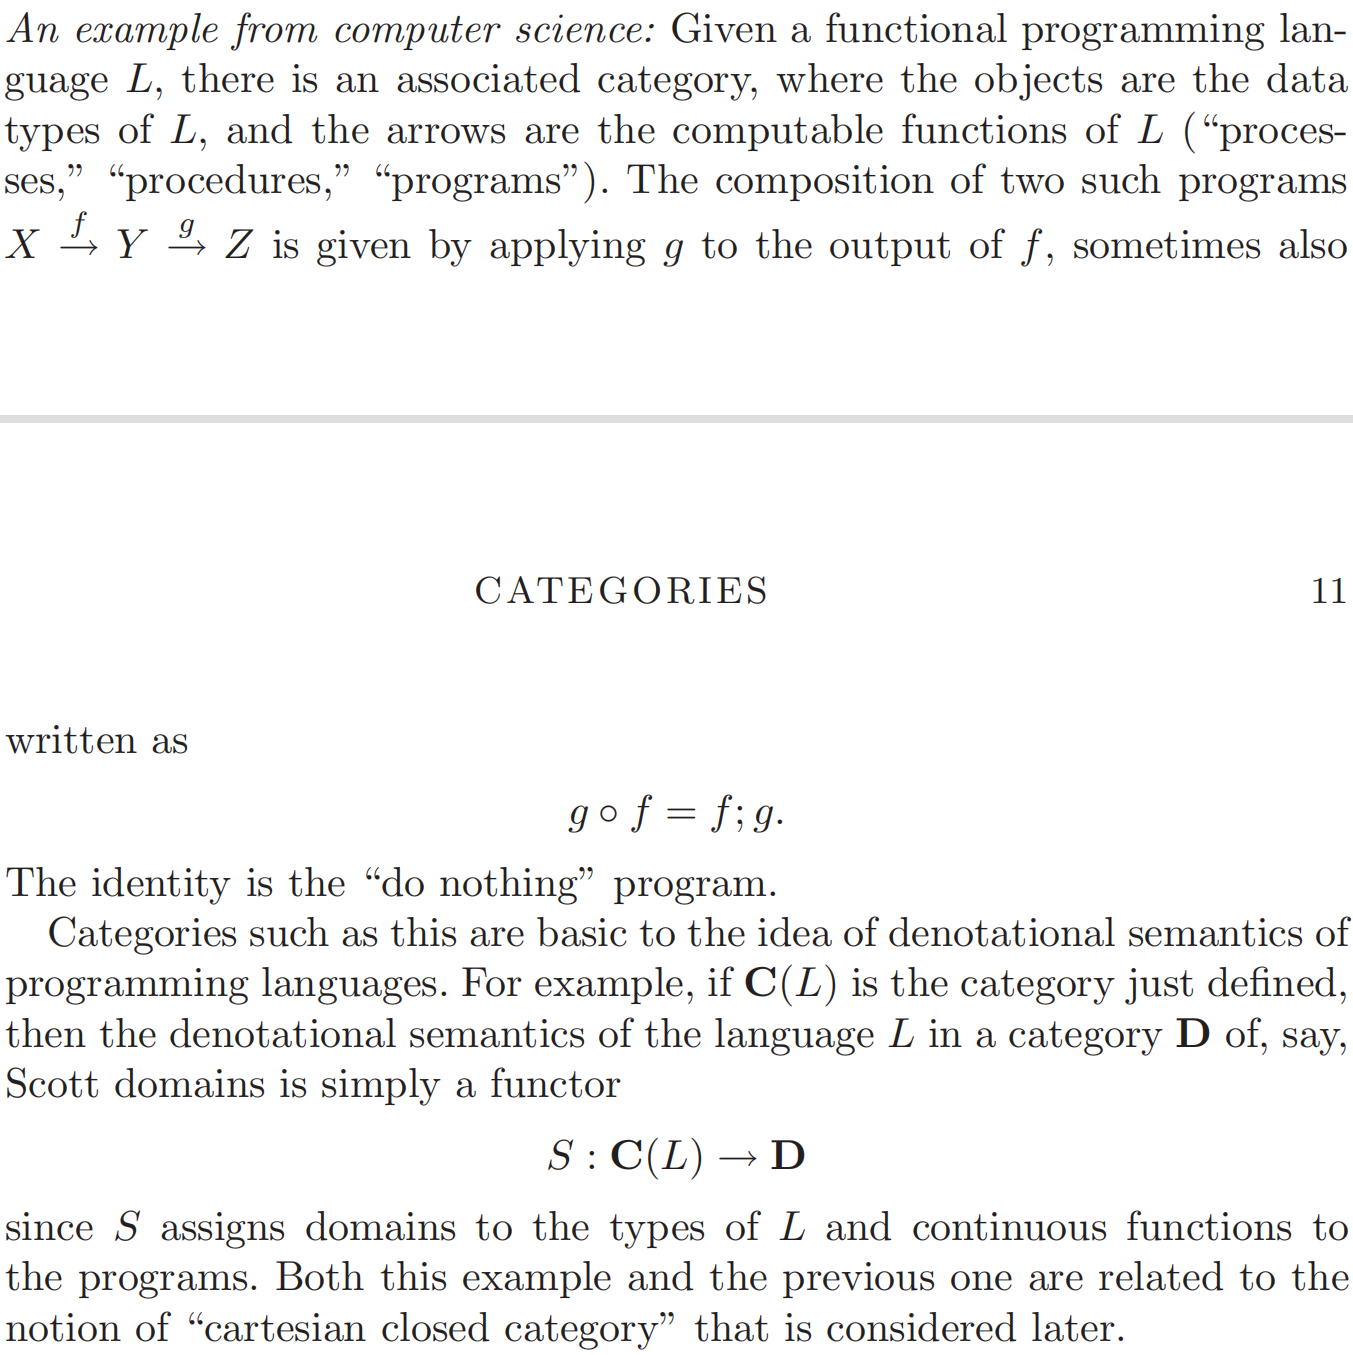
\includegraphics[width=0.7\linewidth]{1.4_11}
		\caption{}
		\label{fig:1}
	\end{figure}
	
	\subsection{Isomorphisms}
	\paragraph{Definition 1.3}
	while there are ``bijective homomorphisms''
	between non-isomorphic posets.
	
	\blue{The inverse must also be homomorphism?}
	
	\paragraph{Theorem 1.6}
	

	\[\red{f,h\in \bar{C}}, \blue{g\circ f,g\circ h\in \bar{D}}.\]
	\begin{centikzcd}[
			remember picture,
			every matrix/.append style={name=arrows}
		]
		X\ar[d,red,"f"']\ar[rd,blue,"g\circ f"]&\\
		C\ar[r,purple,"g"]&D&&\red{\bar{C}}\ar[r,purple,"\bar{g}"] & \blue{\bar{D}} \\
		Y\ar[u,red,"h"]\ar[ru,blue,"g\circ h"']&
	\end{centikzcd}
	%\begin{tikzpicture}[remember picture, overlay]
	%	\def\mid{40}
	%	\draw[red,rounded corners] ([xshift=0pt]arrows.south west) rectangle ([xshift=17.5pt, yshift=15pt]arrows.north west)
	%	node [below left] {$\bar{C}$};
	%\end{tikzpicture}

	If every category (large or small) was isomorphic to a concrete (small) category,
	what make those large?
	
	\blue{The assumption is wrong. Only small categories are isomorphic to a small category.}
	See this: \ref{sec:too_many_arrows}.
	
	\blue{Also see Warning 1.13 that small does not imply concrete and neither is the converse.} 
		
	\paragraph{Remark 1.7}
	\subparagraph{}
	
	\red{What does this mean}
	\begin{figure}[H]
		\centering
		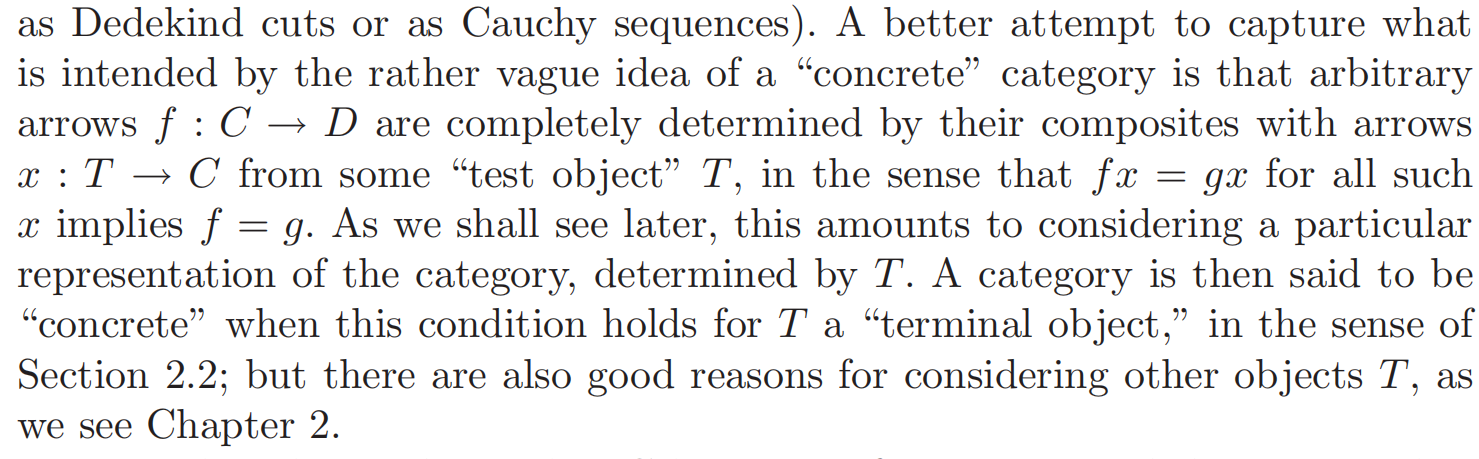
\includegraphics[width=0.7\linewidth]{1.5_1.7}
		\caption{}
		\label{fig:2}
	\end{figure}
	
	\subparagraph{}\label{sec:too_many_arrows}
	\blue{If the arrows in the category is too large to form a set, then it might not be isomorphic to a small category?}
	
	\subsection{Constructions on categories}
	\paragraph{3 The arrow category}
	
	\begin{centikzcd}
		A\ar[r,"g_1"]\ar[d,"f"]&A'\ar[r,"h_1"]\ar[d,"f'"]&A''\ar[d,"f''"]\\
		B\ar[r,"g_2"]&B'\ar[r,"h_2"]&B''
	\end{centikzcd}
	\paragraph{4 Slice category}
	
	\subparagraph{}
	
	\[ \bfC/(-)\colon\bfC\to\mathbf{Cat}\colon C\to\bfC/C\colon g\to g_*. \]
	
	\subparagraph{}
	
	\blue{the forgetful functor $U \colon \mathbf{Cat} \to \mathbf{Sets}$
	that takes a category to its underlying set of objects.}

	Do the objects form a set? Guaranteed?
	\href{https://math.stackexchange.com/questions/750731/is-there-a-category-of-categories}{Is there a category of categories?}
	
	\blue{Yes, because $\mathbf{Cat}$ is defined as the category of \textit{small} categories.
		There is no category of all categories. Likewise, there is no ``set of all sets'' or ``class of all classes''}
	
	\red{But is $\bfC/C$ a small category? If and only if $\bfC$ is small?}
	
	\subparagraph{principal ideal}
	
	the slice category P/p is just the \red{``principal ideal'' (what does this mean? what is down arrow?)} $\downarrow (p)$ of elements $q \in P$
	with $q \le p$.
	
	\paragraph{Example 1.8}
	
	$1=\set{*}$ is mapped to the distinguished point of sets in $\mathbf{Sets}_*$.
	
	\subsection{Free categories}
	\paragraph{Free monoid}
	The Kleene closure of $A$ can be thought as
	\[ \set{\text{Empty word}} \sqcup A \sqcup A\times A \sqcup \dots ,  \]
	where $\times $ is the Cartesian product.
	
	A free monoid can be thought as some monoid isomorphic to the  Kleene closure of some set.
	
	A free monoid can be defined as a monoid whose non-identity elements can be uniquely written as a product of its generating elements?
	
	\paragraph{UMP}
	
	The mapping $i\colon A\to |M(A)|$ must be injection because otherwise there is no monoid
	homomorphism from $M(A)$ to $A^*$, the Kleene closure.
	
	\paragraph{Free category}
	
	\red{Does edges and vertices always form a set?}
	
	\subsection{Foundations: large, small, and locally small}
	
	\paragraph{Definition 1.12}
	
	\subparagraph{The category of sets is locally small}
	
	Given two \textit{sets} $X$ and $Y$,
	an ordered pair $(x,y)\in X\times Y$ can be viewed as an element in $\power\power(X\cup Y)$
	(by Kuratowski's definition).
	Therefore, a function $f\colon X\to Y$ as a subset of $X\times Y$ is an element of $\power\power\power(X\cup Y)$.
	In conclusion, the set of all functions from $X$ to $Y$ is a subset of $\power\power\power(X\cup Y)$,
	and therefore based on the axiom of replacement and power set, it is a (small) set.
	
	\subparagraph{The category of small categories is locally small}
	
	Since the objects and arrows form two sets, so does their disjoint union.
	
	Therefore, a functor can be viewed as a function between two sets, and therefore $\mathbf{Cat}$ is locally small.
	
	\subparagraph{Non-locally small category}
	
	\href{https://mathoverflow.net/questions/3278/whats-a-reasonable-category-that-is-not-locally-small}{Examples}
	
	\subsection{Exercises}
	\paragraph{2}
	\subparagraph{a}
	
	Yes, $\mathbf{Rel}\cong\opp{\mathbf{Rel}}$.
	\subparagraph{b}
	$\mathbf{Sets}$ is not isomorphic to its opposite because
	all terminal objects must be mapped to an initial object as
	a terminal object in the opposite,
	than mapped back to a terminal object.
	
	But there are infinite terminal objects in $\mathbf{Sets}$
	(singletons) and only one initial object (the empty set).
	
	\subparagraph{c}
	
	\blue{For the whole power set it should be true?}
	
	Any subset is mapped to its complement.
	
	This is not necessarily true for a subset of the power set.
	
	\paragraph{3}
	\subparagraph{c}
	There is a bijective monotone function (functor) from a discrete (small) category
	(which is a poset)
	 to a non-discrete poset category of same objects.
	
	But this is not isomorphism.
	
	\paragraph{5}
	
	\[F\colon\bfC/C\to\bfC^{\rightarrow}\]
	is the trivial functor which maps arrows to itself.
	
	\paragraph{6}
	
	\[C/\bfC \cong \opp{(\opp{\bfC}/C)}. \]
	The only difference is the objects are arrows with opposite directions.
	
	\begin{centikzcd}
		X\ar[rr,"a"]\ar[rd,"f"']&&X'\ar[ld,"f'"] \\
		&C\ar[rd,"g'"]\ar[ld,"g"']&\\
		Y\ar[rr,"b"']&&Y'\\
	\end{centikzcd}

	\paragraph{7}
	
	\subparagraph{}
	For any positive integer $n$,
	\[ F\colon\mathbf{Sets}/n\to \mathbf{Sets}^n, \]
	\[ (f\colon X\to \set{a_1,\dots,a_n} )\mapsto (f^{-1}(a_1),\dots,f^{-1}(a_n)).  \]
	\[  (f\to g)\mapsto (f^{-1}(a_1)\to g^{-1}(a_1),\dots, f^{-1}(a_n)\to g^{-1}(a_n)  ) .\]
	
	\begin{enumerate}
		\item 
		First, the image is contained in the codomain.
		
		\item
		It is a functor.
		
		\item \red{It is isomorphism?}
	\end{enumerate}

	\paragraph{8}
	
	In the preorder category $P(\bfC)$,
	any information encoded in the arrows is forgotten,
	only the domain and codomain is kept.
	
	\begin{centikzcd}
		 A \ar[r,bend left=45,"f_1"]\ar [r,"f_2"] \ar[loop left,"1_A"] \ar[loop,in=140,out=220,looseness=10,"i_A"]
		 &B\ar[l,shift left=2,"g"] &C\ar[l,"h"']\\
		 A \ar[r,shift left=1,"f'"] \ar[loop left,"1_A"] 
		 &B\ar[l,shift left=1,"g'"] &C\ar[l,"h'"']\\
	\end{centikzcd}

	$P(1_A)=P(i_A)=1_A, P(f_1)=P(f_2)=f'$.
	
	Since any functor preserves domain and codomain,
	any functor can be mapped as an arrow between two preorder sets.
	
	For example, given two categories $\bfC,\bfD$,
	if the functor $F$ maps \textit{any} arrow in $\bfC$ $(X\to Y)$ to \textit{an} arrow in $\bfD$ $(F(X)\to F(Y))$,
	then the it maps \textit{the} arrow in $P(\bfC)$ $(X\to Y)$ to \textit{the} arrow in $P(\bfD)$ $(F(X)\to F(Y))$.
	
	The identity is preserved since $A\le A$, the composite is preserved due to the transitivity $A\le B\land B\le C\implies A\le C$.
	
	Let $I$ be the inclusion, then $P\circ I=1$ but $I\circ P\ne 1$.
	
	\paragraph{9}
	\subparagraph{c}
	
	\begin{eqlong}
		a\to a&: 1_a,\\
		a\to b&: e,\\
		b\to b&: 1_b,\\
		b\to c&:f,\\
		c\to c&:1_c,\\
		a\to c&:f\circ e,g,\\
	\end{eqlong}

	\subparagraph{d}
	The only arrow related to $d$ is $1_d$.
	
	\[a\to a:1_a,(he)^n, (gfe)^n,\]
	\[b\to b:1_b,(eh)^n, (egf)^n,\]
	\[c\to c:1_c,(feg)^n.\]
	\[a\to b:e\circ (a\to a); b\to a: (h \lor gf)\circ (b\to b).\]
	
	\paragraph{10}
	
	\red{Can you have a directed graph with only 1 vertex, but 6 edges on the same vertex?
	or only 2 vertices and 3 edges for each direction connecting these?}

	\paragraph{11}
	\subparagraph{b}
	Assume $\forall A\in \mathbf{Sets}\, \exists! i_A\colon A \to |M(A)|$ as UMP,
	then \[ \forall (f\colon A\to B)\, \exists! i_B\circ f\, \exists! M(f) \]
	such that the following diagram commutes.
	\begin{centikzcd}
		\mathbf{Mon}& M(A)\ar[r,red,dashed,"\exists!M(f)"]&M(B)\\
		\mathbf{Sets}& \vert M(A) \vert \ar[r,red,"|M(f)|"]& \vert M(B)\vert \\
		&A\ar[r,"f"]\ar[ru,red,"i_B\circ f"]\ar[u,red,"i_A"]& B\ar[u,"i_B"]
	\end{centikzcd}

	Let $f=1_A$, and $B=A$.
	Since $1_{|M(A)|}\circ i_A = i_A\circ 1_A$ and $|1_{M(A)}|=1_{|M(A)|}$,
	therefore $M(1_A)=1_{M(A)}$.
	
	Associativity:
	\begin{centikzcd}
		\mathbf{Mon}& M(A)\ar[r,red,dashed,"\exists!M(f)"]&M(B)\ar[r,dashed,blue,"\exists! M(g)"]&M(C)\\
		\mathbf{Sets}& \vert M(A) \vert \ar[r,red,"|M(f)|"]& \vert M(B)\vert \ar[r,blue,"|M(g)|"]& \vert M(C)\vert \\
		&A\ar[r,"f"']\ar[ru,red,"i_B\circ f"']\ar[u,red,"i_A"]& B\ar[u,blue,"i_B"]\ar[ru,blue,"i_C\circ g"']\ar[r,"g"']&C\ar[u,"i_C"]
	\end{centikzcd}

	\paragraph{14}
	\red{TODO}
	
	\section{Abstract structures}
	
	\subsection{Epis and monos}
	\paragraph{Example 2.3}
	\subparagraph{Prove $h$ monic implies $|h|$ monic}
	
	\[ h\bar{x}\ne h\bar{y}\implies|h|x\ne|h|y, \]
	due to UMP of $M(1)$.
	(If $|h|x=|h|y$, then there exists non-unique maps $h\bar{x}, h\bar{y}$ corresponding it,
	which contradicts UMP.)
	
	
	\subparagraph{Converse}
	
	If $f,g : X \to M$ are any distinct
	homomorphisms, then $|f|, |g| : |X|\to|M|$ are distinct functions.
	The converse is true, only if there is a monoid homomorphism corresponding to the underlying function.
	This is to say, function to monoid homomorphism mapping is injective but not surjective.
	
	\paragraph{Example 2.4}
	
	Because there is at most 1 arrow between 2 objects!
	\subsubsection{Sections and retractions}
	\paragraph{Definition 2.7}
		
	$A$ is ``smaller'' than $X$.
	
	\blue{Functors preserve split epis and split
	monos, but do not preserve all the epis.}

	\paragraph{Projective}
	\red{What does projective mean?}
	
	\subparagraph{Epi into projective object splits}
	
	Let $P$ be the projective object and $e\colon E \twoheadrightarrow P$ the epi.
	Since $1_P$ must exist, therefore
	by definition of projective object, $\exists m$ such that
	\begin{centikzcd}
		&E\ar[d,two heads,"e"]\\
		P\ar[ru,dashed,tail,"\exists m"] \ar[r,"1_P" ] & P\\
	\end{centikzcd}
	Therefore $e$ splits and $m$ is mono
	(by definition of split epi).
	
	\subparagraph{More free}
	Projective objects may be thought of as having a more ``free'' structure, thus
	permitting ``more arrows''.
	
	I guess this means: for any epi and any arrow from a projective object sharing the codomain,
	there must be another arrow from the projective object to the domain of the epi,
	so there will be ``more'' arrows than ``necessary''.
	
	\subparagraph{AC vs projective}
	
	\blue{If all epis are split, then all objects are projective.} Because for any epi $e\colon E\twoheadrightarrow X$
	there is a mono $m\colon X\rightarrowtail E$ such that $em=1_X$, therefore for any $f\colon P \to X$,
	there must be $\bar{f}=m\circ f$ such that the following diagram commutes.
	\begin{centikzcd}
		&E\ar[rd,two heads,"e"]&\\
		P\ar[r,"f"]\ar[ru,dashed,"m\circ f"]&X\ar[r,"1_X"]\ar[u,tail,"m"]&X
	\end{centikzcd}

	\red{It follows that
		free objects in many (but not all!) categories of algebras then are also projective.}

	\subparagraph{Retract of projective object}
	
	Let $R$ be a retract of a projective object $P$,
	and let $rs=1_R$.
	Then given any epi $e\colon E\twoheadrightarrow X$, 
	and any $f\colon R\to X$, the following diagram must commute.
	\begin{centikzcd}
		&&E\ar[d,red,two heads,"\forall e"]\\
		&P\ar[r,red,"f\circ r"]\ar[ru,dashed,red,"\exists \overline{f\circ r}"]\ar[d,two heads,"r"]&X\\
		R\ar[ru,tail,"s"]\ar[r,"1_R"]&R\ar[ru,purple,"\forall f"'] &
	\end{centikzcd}

	And therefore $f$ lifts across $e$ to $\overline{f\circ r} \circ s$.
	
	\subsection{Initial and terminal objects}
	
	\paragraph{Example 2.11}
	\subparagraph{3 Rings}
	In $\mathbf{Rings}$ (commutative with unit), the ring $\inte$ of integers is initial.
	
	For any finite rings, they might not be homomorphic to other finite rings of different size (\eg, $\field_q$).
	
	$\inte$ is the smallest infinite ring. Since $0$ must be mapped to $0$ and so is $1$, there exists a unique ring homomorphism
	from $\inte$.
	\subsection{Generalized elements}
	
	\paragraph{Ultrafilter}
	a filter $F$ is an ultrafilter just if for every element $b \in B$, either $b \in F$ or $\neg b \in F$,
	and not both (exercise!).
	
	\paragraph{Prime ideal}
	Ring homomorphisms $A \to Z$ into the initial ring $Z$ play an analogous and
	equally important role in algebraic geometry. They correspond to so-called prime
	ideals, which are the ring-theoretic generalizations of ultrafilters.
	\paragraph{Example 2.12}
	\subparagraph{3}
	\[f=g\iff f1_C=g1_C.\]
	\paragraph{Example 2.13}
	\red{$\Hom(X, -)$ is always a functor, and functors always preserve isos.}
	\paragraph{Example 2.14}
	\subparagraph{Natural number is the revealing object}
	
	
	\begin{centikzcd}
		\mathbf{Mon}& M(1)\ar[r,dashed,"\exists \bar{x}"]&M\\
		\mathbf{Sets}& \vert M(1) \vert \ar[r,"|\bar{x}|"]& \vert M\vert \\
		&\set{*} \ar[ru,"\forall x"']\ar[u,"i"]&
	\end{centikzcd}

	For any $x\in |M|$, there is a function $x\colon *\mapsto x$.
	To make the diagram commute, $|\bar{x}|\big( i(*)\big)= x$.
	
	This uniquely corresponds to a monoid homomorphism $\bar{x}\colon i(*)\mapsto x$.
	Therefore, every element in $|M|$ can be reached by a monoid homomorphism from $M(1)$.
	And $\nat$ is isomorphic to $M(1)$.
	\subparagraph{Bijection}
	From above, we clearly see that different $x$ correspond to different monoid homomorphism $\bar{x}\colon i(*)\mapsto x$,
	and exactly one for each.
	Therefore \[\card{\Hom_{\mathbf{Sets}}(1,|M|)}\le \card{\Hom_{\mathbf{Mon}}(M(1),|M|)}.\]
	
	On the other hand, for any monoid homomorphism $f\colon M(1)\to M$,
	there is uniquely $x=|f|\circ i$ which makes the diagram commute.
	Different $f$ must correspond to different $x$, otherwise it contradicts the UMP axiom.
	
	\subparagraph{Bijection in general}
	
	\begin{def*}[universal property]
		Let $F\colon \bfC\to \bfD$ be a functor between categories $\bfC$ and $\bfD$,
		and let $X\in\ob(\bfD), A,A'\in\ob(\bfC)$.
		
		A \textbf{universal morphism} from $X$ to $F$ is a unique pair $(A,u\colon X\to F(A))$ in $D$
		such that any morphism of the form $f\colon X\to F(A')$ in $D$, there \textit{exists a unique} morphism
		$h\colon A\to A'$ in $C$ such that $f=F(h)\circ u$, \ie, the following diagram commutes:
		\begin{centikzcd}
			\bfC & \blue{A} \ar[dashed,r,"\exists ! h"] & A'\\
			\bfD & F(\blue{A}) \ar[dashed,r,"\exists F(h)"] & F(A')\\
			& X \ar[u,red,"u"] \ar[ur,"\forall f"'] &
		\end{centikzcd}
	\end{def*}

	\begin{prop}
		Given two locally small categories $\bfC$ and $\bfD$,
		if $(A,u\colon X\to F(A))$ is a universal morphism,
		then $\forall A'\in \ob(\bfC)$ there is a bijection for hom-sets
		\[ \Hom_\bfC(A,A')\cong \Hom_\bfD(X,F(A')). \]
	\end{prop}
	\begin{proof}
		From the definition of universal morphism,
		there is a unique $h\in \Hom_\bfC(A,A')$ corresponding
		each $f\in \Hom_\bfD(X,F(A'))$, and let the mapping be
		\[ G\colon\Hom_\bfD(X,F(A'))\to  \Hom_\bfC(A,A')\colon f\to h  \]
		such that the definition diagram commutes.
		
		Conversely, for any $g\in \Hom_\bfC(A,A')$, there exists a unique
		morphism $ F(g) \circ u $ such that the definition diagram commutes,
		therefore
		\[ G'\colon\Hom_\bfC(A,A')\to  \Hom_\bfD(X,F(A')) \colon g\to F(g) \circ u   \]
		is another mapping.
		
		Since the diagram commutes, they must be inverse, \ie,
		\[ GG'=1, G'G=1. \]
	\end{proof}
	\begin{rem*}
		Different $h$ corresponds to different $f$
		because otherwise it contradicts the universal property.
		
		Different $f$ corresponds to different $h$
		because the composite $F(g)\circ u$ is uniquely determined by its components $F(g)$ and $u$.
		And there is no other morphism $X\to F(A')$ that makes the diagram commute.
	\end{rem*}
	
	
	\subsection{Products}
	\paragraph{Arrows out of the product}
	\red{To be sure, they are related to the notion of an
	``exponential'' $Y^B$, via ``currying'' $\lambda f : A \to Y^B$; we discuss this further in
	Chapter 6.}
	\subsection{Examples of products}
	\paragraph{3}
	\red{Check properties}
	\paragraph{4}
	Greatest lower bound is just $\min$ function in totally ordered set.
	
	\paragraph{6 Lambda calculus}
	
	\red{type theory}
	
	\red{closed terms = no free variables?}
	
	\red{$\beta\eta$-equivalence means $\lambda x.x=\lambda y.y$?}
	\paragraph{Remark 2.18 ``Curry--Howard'' correspondence}
	
	\red{Functor from category of proofs to category of types}
	
	\subsection{Categories with products}
	
	
	
	\subsection{Hom-sets}
	\subsection{Exercises}
\end{document}